\hypertarget{introduction}{%
\section{Introduction}\label{introduction}}

To complete this activity, I implemented a basic access control list
using Python. This is modelled after the Windows implementation where
the resource owner decides permissions, unlike the Unix-like approach
which take a role-based approach to access control. Consequently, this
is a discretionary access control (DAC) system.

Note that unlike traditional access-control implementations, this only
stores permission information for as long as the program is running
(i.e.~there is no persistent storage mechanism). This means that if the
program ever crashes or stops functioning for any reason, the permission
associated with each file is lost (but not the files themselves).
Additionally, access is only enforced using the program and is,
therefore, more like a prototype rather than a complete implementation.
The reason for this is because Linux (which is what was being used to
run this program) already has its own access control system, and mixing
them could potentially break something. While this does mean that any
user outside of the program can read any resource contents, it will be
assumed that the Python script running the implementation is the only
way to access the files for simplicity.

\hypertarget{functionality}{%
\subsection{Functionality}\label{functionality}}

This implementation supports a few different (basic) actions - creating
a resource, reading a resource, writing to a resource, setting who can
read a resource, and changing the resource's owner. By default, the
program is signed into the user ``alice'' by default. This is just
because the program needs someone signed in because users don't have
usernames and passwords (though you can imagine that in a full
implementation this would be required).

\begin{figure}
\centering
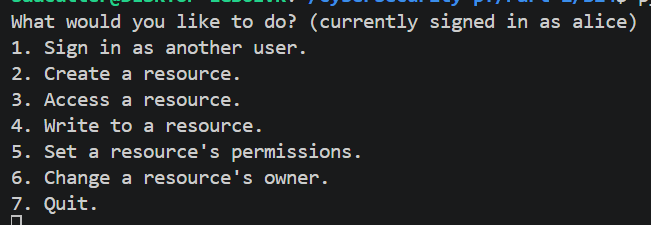
\includegraphics{demonstration/default.png}
\caption{default}
\end{figure}

Creating a resource is the most basic action. This just creates an empty
file and associates it with the user. This action requires the resource
name to be defined by the user.

\begin{figure}
\centering
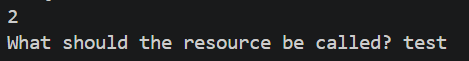
\includegraphics{demonstration/create.png}
\caption{create}
\end{figure}

Now that the resource has been created, it can be read by the resource
owner (or anyone with the correct permissions).

\begin{figure}
\centering
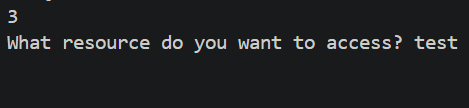
\includegraphics{demonstration/read.png}
\caption{read}
\end{figure}

This resource is currently empty, so nothing was returned. This is the
perfect opportunity to write some data to the file.

\begin{figure}
\centering
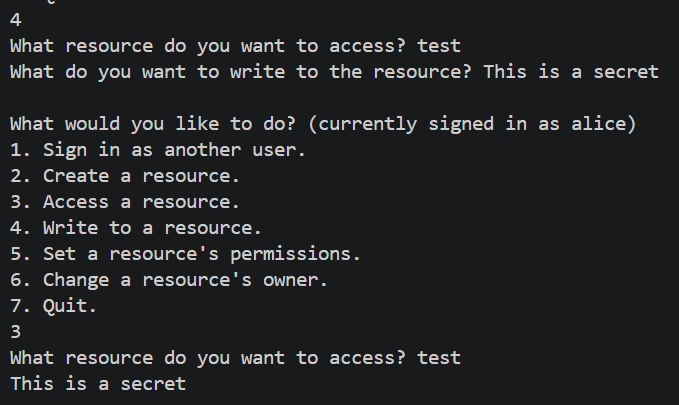
\includegraphics{demonstration/write.png}
\caption{write}
\end{figure}

Now that the writing capabilities have been confirmed and the data can
be read, testing that no one else can read it should be the next option.
This requires another user (let's call them ``bob'') to be signed into
and the previously created file to try and be read.

\begin{figure}
\centering
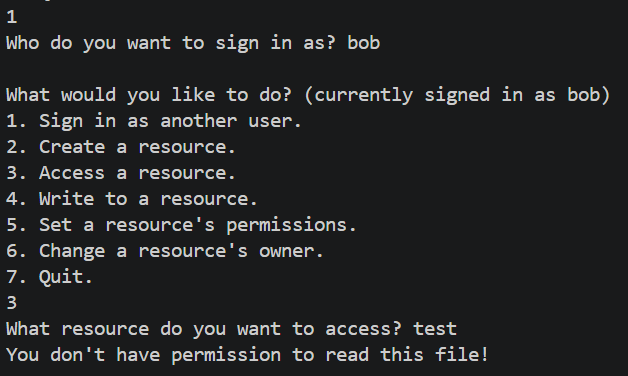
\includegraphics{demonstration/read_denial.png}
\caption{read\_denial}
\end{figure}

This has confirmed that the permissions to file's have been confirmed.
Now that the basic functionality has all been confirmed, trying to
change the resource's owner is the next action to try. To do this, the
\texttt{test} resource created by Alice will be transferred to Bob.

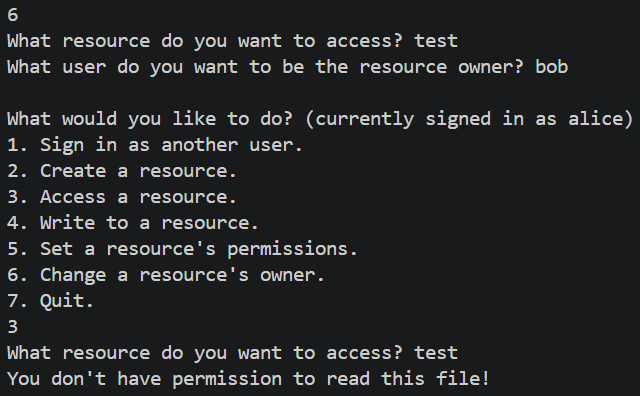
\includegraphics{demonstration/change_owner_alice.png}
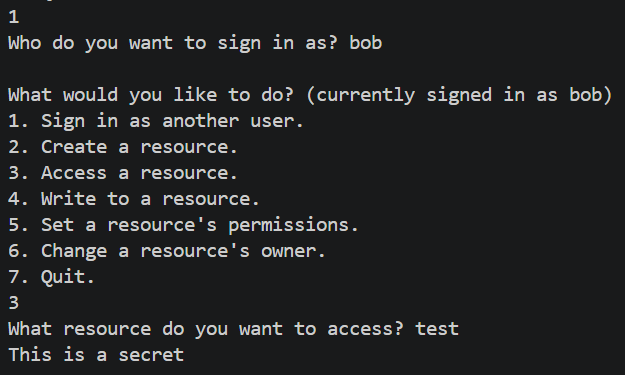
\includegraphics{demonstration/change_owner_bob.png}

Now that Bob owns the file, the permissions to read the file (but not
write the file) can be given to Alice.

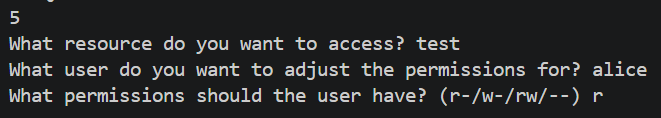
\includegraphics{demonstration/change_permissions_bob.png}
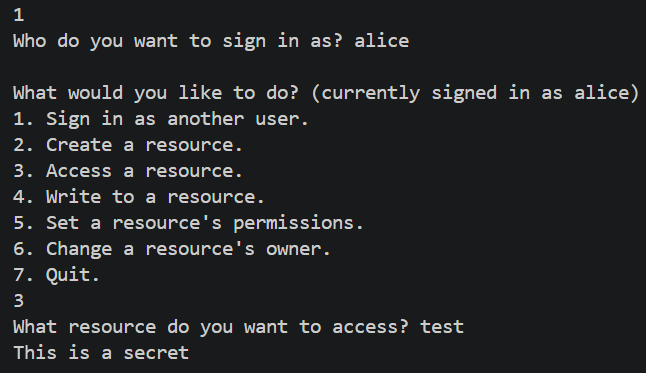
\includegraphics{demonstration/change_permissions_alice.png}

However, trying to read this resource from a third user (Charlie) still
returns a permission error, as expected.

\begin{figure}
\centering
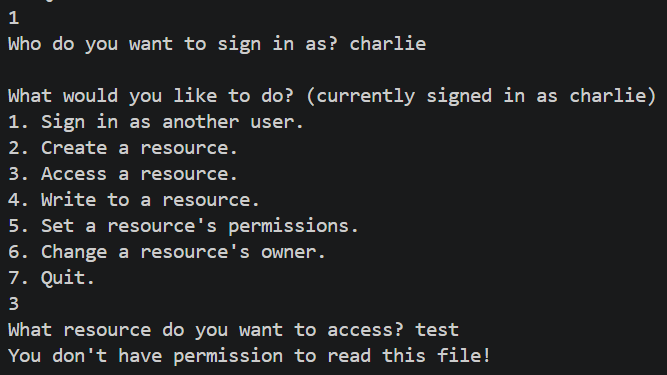
\includegraphics{demonstration/change_permissions_charlie.png}
\caption{permissions\_charlie}
\end{figure}

This demonstration has showcased a minimal access control
implementation, showing how resource permissions can be changed and
shared around to other users.
